%%%%%%%%%%%%%%%%%%%%%%
\begin{frame}{Naming Mechanism}
\vskip 0.7cm
Now we have found the communities, we can be interested in knowing:
\begin{itemize}
	\item the kind of relationship among the vertices
	\item the most important characteristics of the community
	\item the common attributes of the nodes 
\end{itemize}
\vskip 0.8cm
For this reason the authors propose an algorithm to extrapolate this information.
\end{frame}

%%%%%%%%%%%%%%%%%%%%%%
\begin{frame}{Naming Mechanism}
\vskip 0.5cm
The main idea is to take advantage of the social structure of the network in which we have several hubs.
\vskip 0.3cm
 They are \textbf{central entities} in the communities and they put important impacts on the overall formation and development of the given community.
 \vskip 0.3cm
 We can order them using some types of centrality such as:
 \begin{itemize}
 	\item degree
	\item betweenness
	\item Page Rank
	\item closeness
	\item eigenvector
 \end{itemize}

 \end{frame}
 
 %%%%%%%%%%%%%%%%%%%%%%
\begin{frame}{CentralEntityResolution}
\vskip 0.5cm

 Now we sort the nodes according to descending order and we choose the central ones according to the following algorithm.
 \begin{center}
	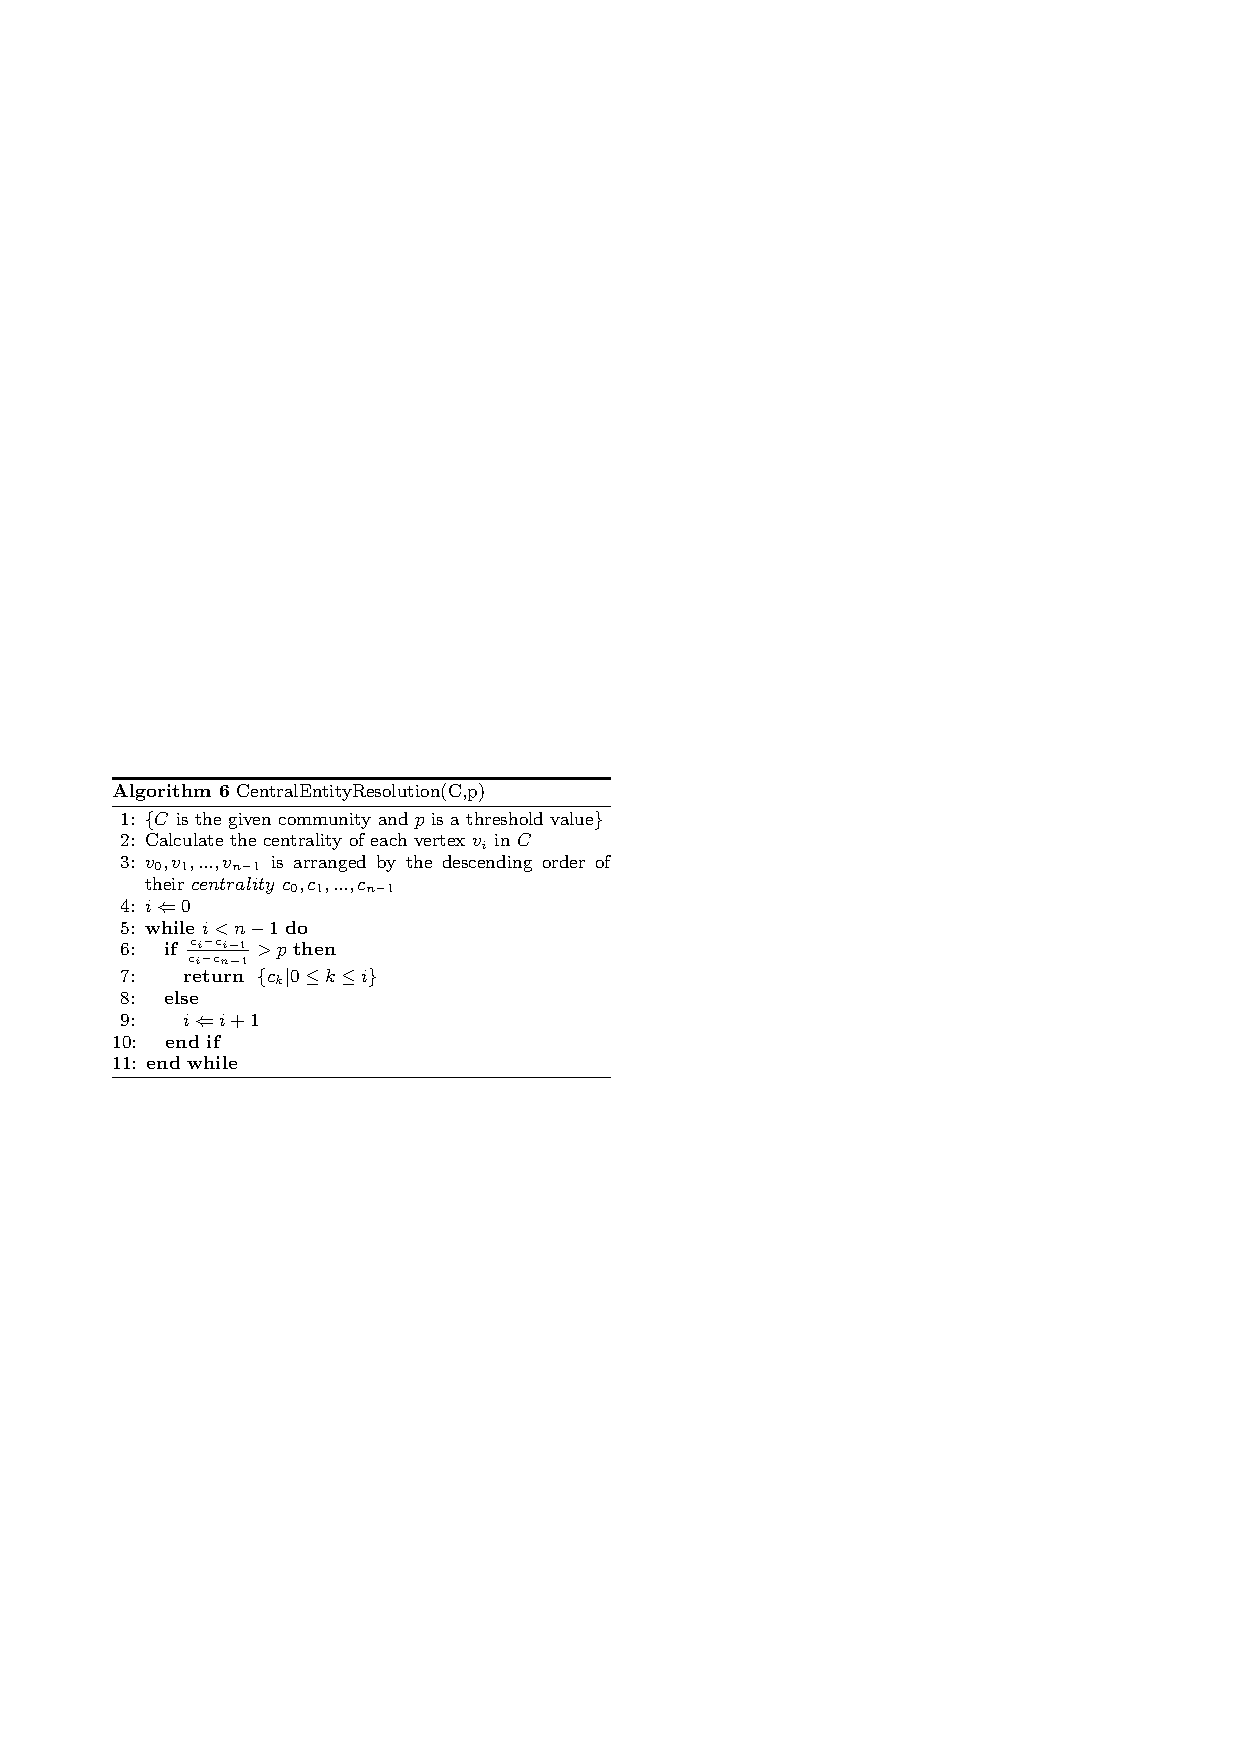
\includegraphics[height=5.5cm]{images/centralEntityResolution.pdf}
\end{center}
\end{frame}


 %%%%%%%%%%%%%%%%%%%%%%
\begin{frame}{NamingCommunity}

 Finally we can associate their attributes to each community.
 \begin{center}
	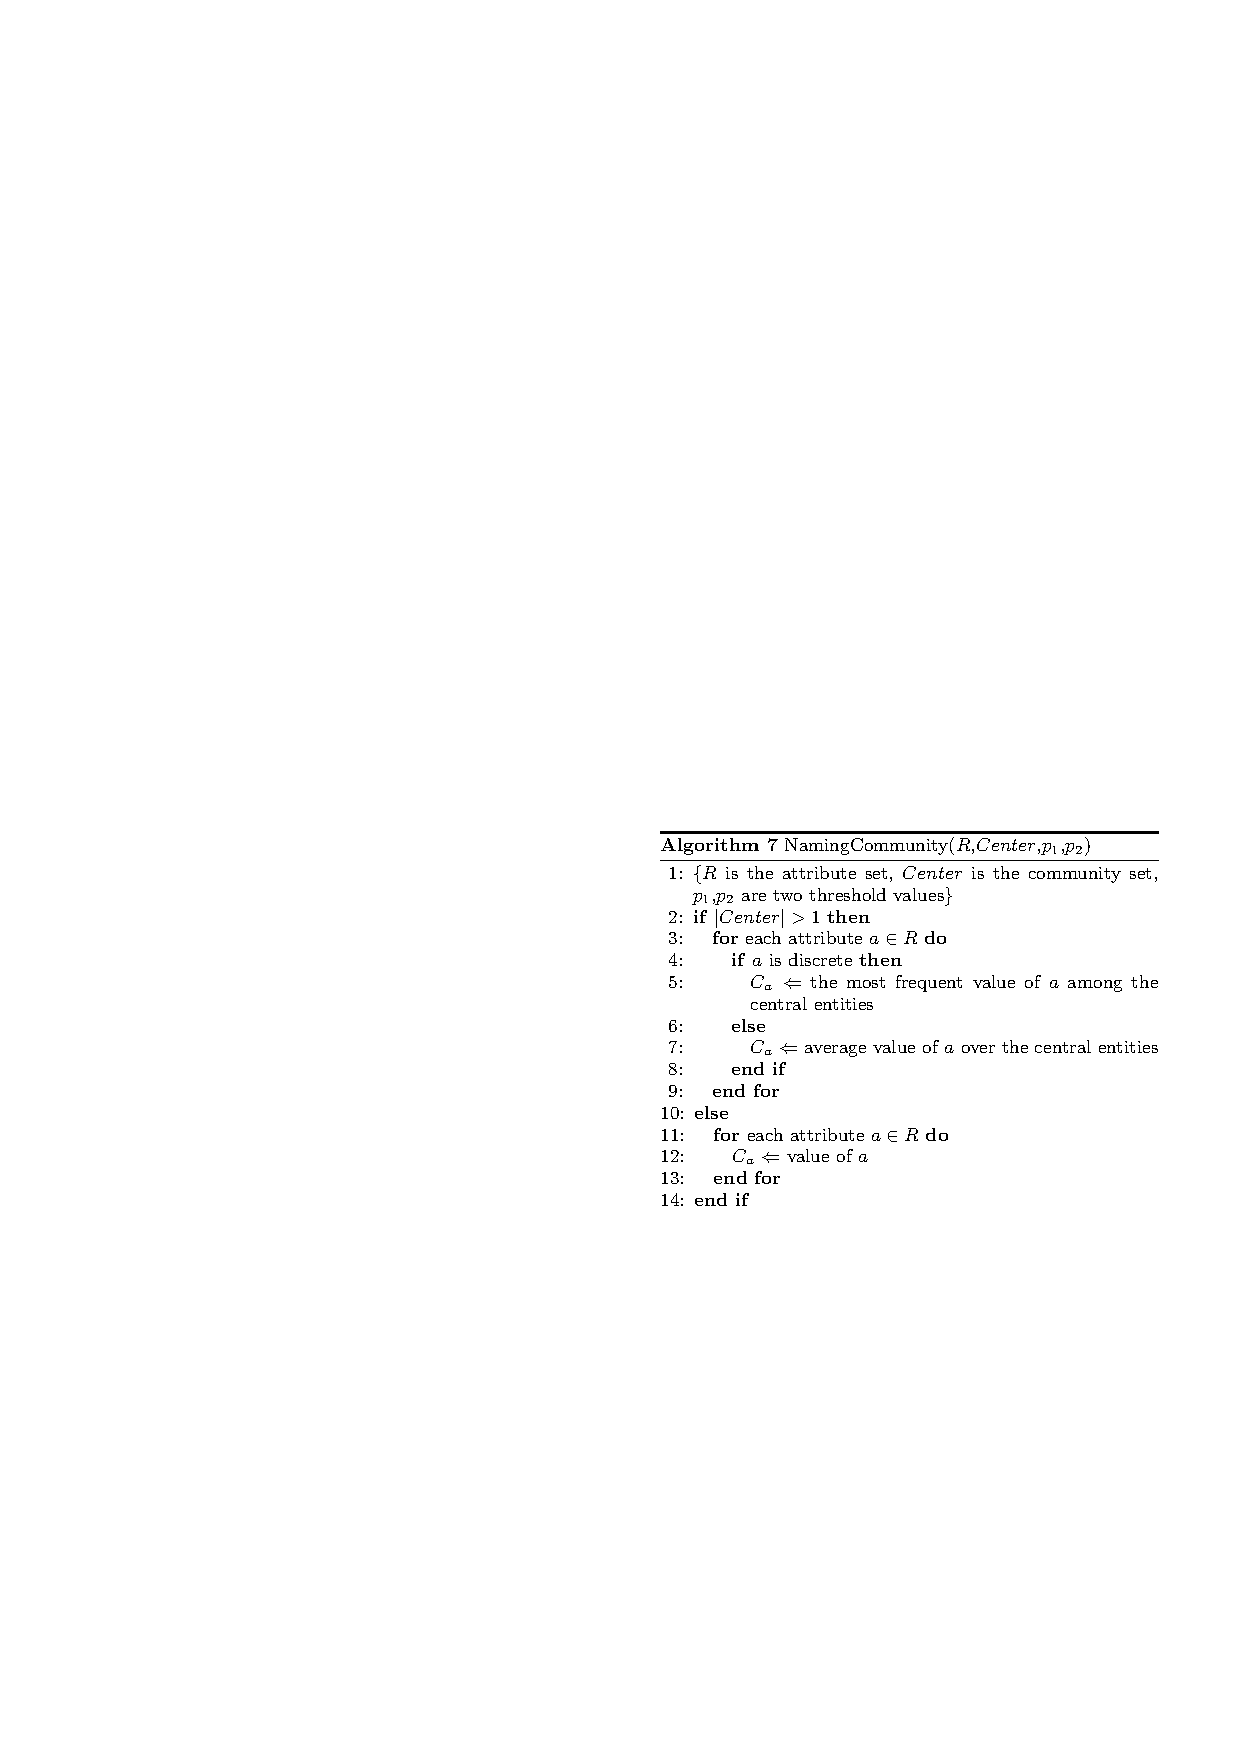
\includegraphics[height=6.7cm]{images/namingCommunity1.pdf}
\end{center}
\end{frame}

\begin{frame}{NamingCommunity}
 \begin{center}
	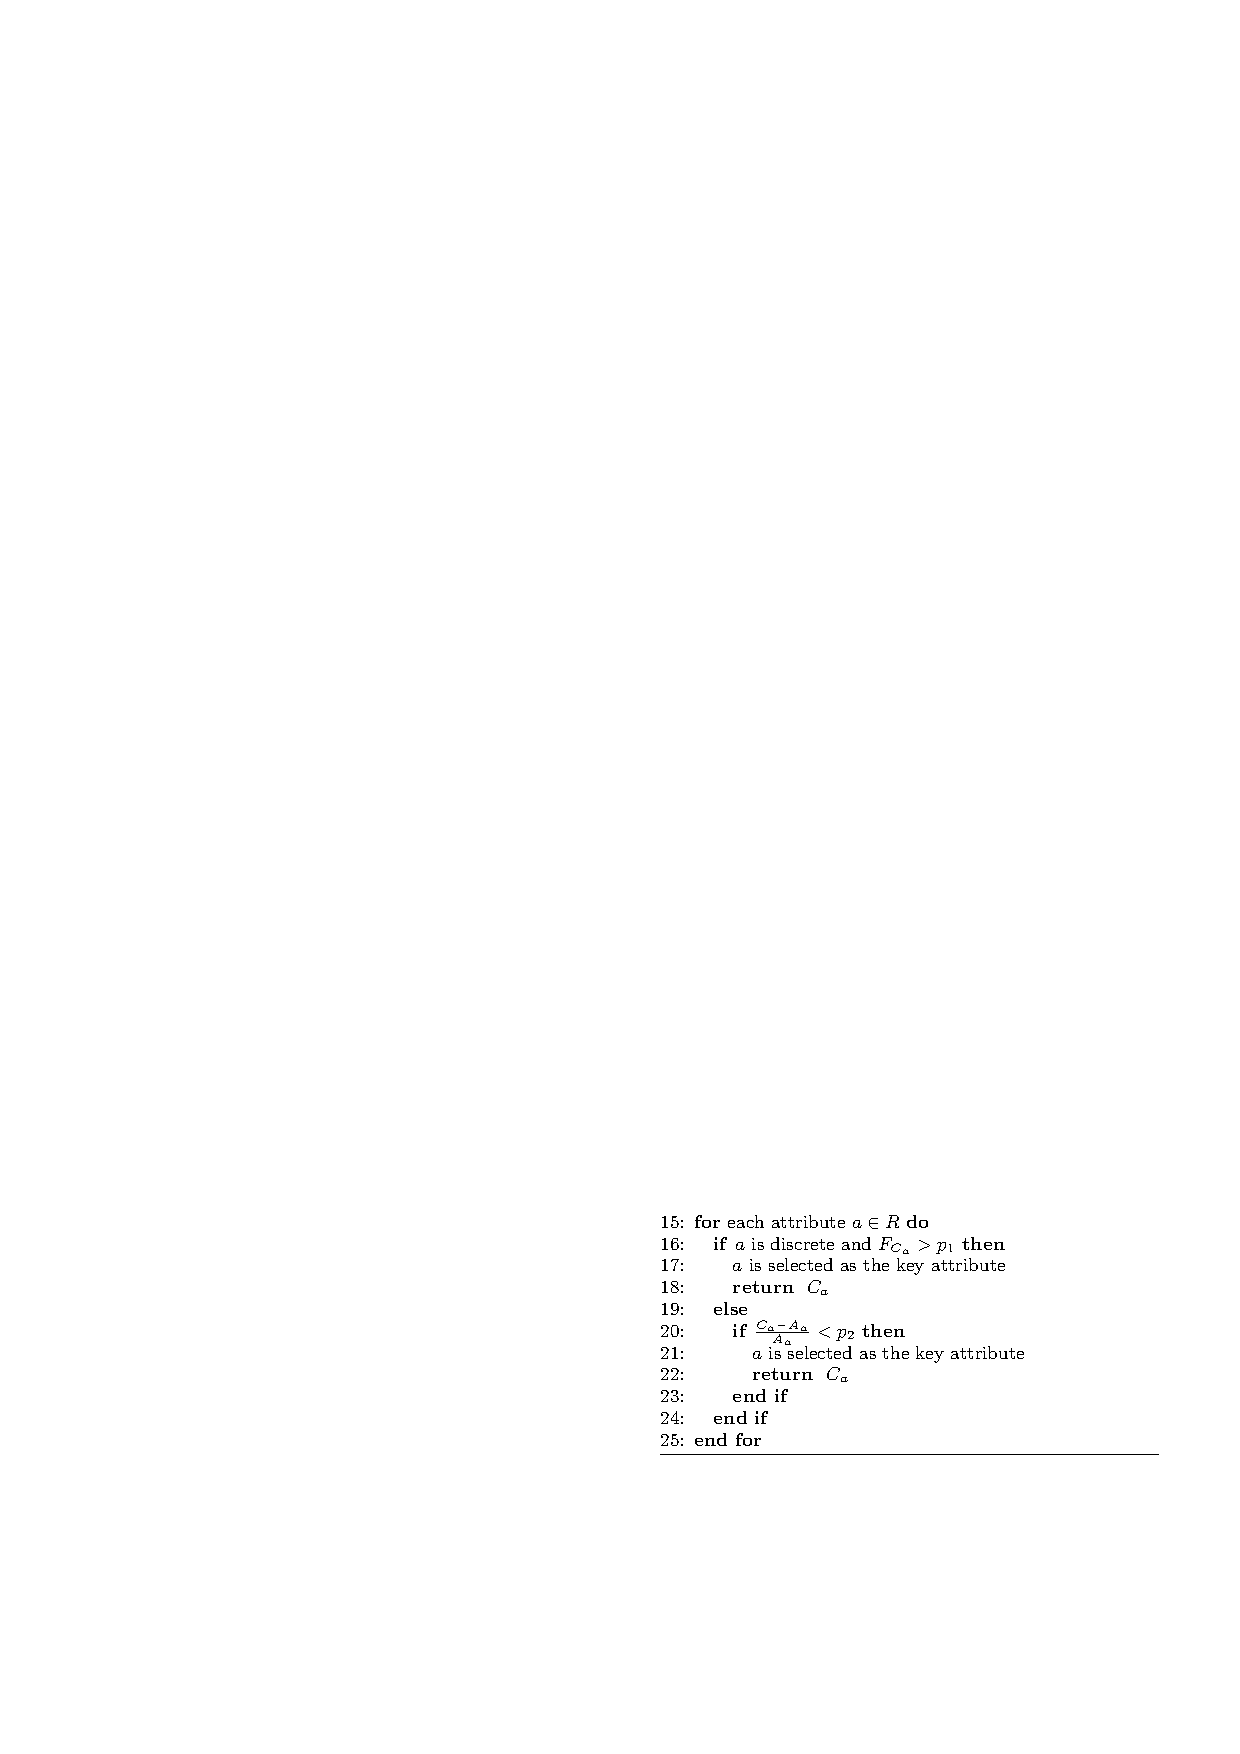
\includegraphics[height=5cm]{images/namingCommunity2.pdf}
\end{center}
\end{frame}
